\documentclass[journal,12pt,twocolumn]{IEEEtran}

\usepackage{setspace}
\usepackage{gensymb}
\singlespacing
\usepackage[cmex10]{amsmath}

\usepackage{amsthm}

\usepackage{mathrsfs}
\usepackage{txfonts}
\usepackage{stfloats}
\usepackage{bm}
\usepackage{cite}
\usepackage{cases}
\usepackage{subfig}

\usepackage{longtable}
\usepackage{multirow}

\usepackage{enumitem}
\usepackage{mathtools}
%\usepackage{steinmetz}
\usepackage{tikz}
\usepackage{circuitikz}
\usepackage{verbatim}
%\usepackage{tfrupee}
\usepackage[breaklinks=true]{hyperref}
\usepackage{graphicx}
\usepackage{tkz-euclide}

\usetikzlibrary{calc,math}
\usepackage{listings}
    \usepackage{color}                                            %%
    \usepackage{array}                                            %%
    \usepackage{longtable}                                        %%
    \usepackage{calc}                                             %%
    \usepackage{multirow}                                         %%
    \usepackage{hhline}                                           %%
    \usepackage{ifthen}                                           %%
    \usepackage{lscape}     
\usepackage{multicol}
\usepackage{chngcntr}

\DeclareMathOperator*{\Res}{Res}

\renewcommand\thesection{\arabic{section}}
\renewcommand\thesubsection{\thesection.\arabic{subsection}}
\renewcommand\thesubsubsection{\thesubsection.\arabic{subsubsection}}

\renewcommand\thesectiondis{\arabic{section}}
\renewcommand\thesubsectiondis{\thesectiondis.\arabic{subsection}}
\renewcommand\thesubsubsectiondis{\thesubsectiondis.\arabic{subsubsection}}


\hyphenation{op-tical net-works semi-conduc-tor}
\def\inputGnumericTable{}                                 %%

\lstset{
%language=C,
frame=single, 
breaklines=true,
columns=fullflexible
}
\begin{document}


\newtheorem{theorem}{Theorem}[section]
\newtheorem{problem}{Problem}
\newtheorem{proposition}{Proposition}[section]
\newtheorem{lemma}{Lemma}[section]
\newtheorem{corollary}[theorem]{Corollary}
\newtheorem{example}{Example}[section]
\newtheorem{definition}[problem]{Definition}

\newcommand{\BEQA}{\begin{eqnarray}}
\newcommand{\EEQA}{\end{eqnarray}}
\newcommand{\define}{\stackrel{\triangle}{=}}
\bibliographystyle{IEEEtran}
\raggedbottom
\setlength{\parindent}{0pt}
\providecommand{\mbf}{\mathbf}
\providecommand{\pr}[1]{\ensuremath{\Pr\left(#1\right)}}
\providecommand{\qfunc}[1]{\ensuremath{Q\left(#1\right)}}
\providecommand{\sbrak}[1]{\ensuremath{{}\left[#1\right]}}
\providecommand{\lsbrak}[1]{\ensuremath{{}\left[#1\right.}}
\providecommand{\rsbrak}[1]{\ensuremath{{}\left.#1\right]}}
\providecommand{\brak}[1]{\ensuremath{\left(#1\right)}}
\providecommand{\lbrak}[1]{\ensuremath{\left(#1\right.}}
\providecommand{\rbrak}[1]{\ensuremath{\left.#1\right)}}
\providecommand{\cbrak}[1]{\ensuremath{\left\{#1\right\}}}
\providecommand{\lcbrak}[1]{\ensuremath{\left\{#1\right.}}
\providecommand{\rcbrak}[1]{\ensuremath{\left.#1\right\}}}
\theoremstyle{remark}
\newtheorem{rem}{Remark}
\newcommand{\sgn}{\mathop{\mathrm{sgn}}}
\providecommand{\abs}[1]{\left\vert#1\right\vert}
\providecommand{\res}[1]{\Res\displaylimits_{#1}} 
\providecommand{\norm}[1]{\left\lVert#1\right\rVert}
%\providecommand{\norm}[1]{\lVert#1\rVert}
\providecommand{\mtx}[1]{\mathbf{#1}}
\providecommand{\mean}[1]{E\left[ #1 \right]}
\providecommand{\fourier}{\overset{\mathcal{F}}{ \rightleftharpoons}}
%\providecommand{\hilbert}{\overset{\mathcal{H}}{ \rightleftharpoons}}
\providecommand{\system}{\overset{\mathcal{H}}{ \longleftrightarrow}}
	%\newcommand{\solution}[2]{\textbf{Solution:}{#1}}
\newcommand{\solution}{\noindent \textbf{Solution: }}
\newcommand{\cosec}{\,\text{cosec}\,}
\providecommand{\dec}[2]{\ensuremath{\overset{#1}{\underset{#2}{\gtrless}}}}
\newcommand{\myvec}[1]{\ensuremath{\begin{pmatrix}#1\end{pmatrix}}}
\newcommand{\mydet}[1]{\ensuremath{\begin{vmatrix}#1\end{vmatrix}}}
\numberwithin{equation}{subsection}
\makeatletter
\@addtoreset{figure}{problem}
\makeatother
\let\StandardTheFigure\thefigure
\let\vec\mathbf
\renewcommand{\thefigure}{\theproblem}
\def\putbox#1#2#3{\makebox[0in][l]{\makebox[#1][l]{}\raisebox{\baselineskip}[0in][0in]{\raisebox{#2}[0in][0in]{#3}}}}
     \def\rightbox#1{\makebox[0in][r]{#1}}
     \def\centbox#1{\makebox[0in]{#1}}
     \def\topbox#1{\raisebox{-\baselineskip}[0in][0in]{#1}}
     \def\midbox#1{\raisebox{-0.5\baselineskip}[0in][0in]{#1}}
\vspace{3cm}
\title{EE3025 ASSIGNMENT- 1}
\author{VARUN SM - EE18BTECH11030}
\maketitle
\newpage
\bigskip
\renewcommand{\thefigure}{\theenumi}
\renewcommand{\thetable}{\theenumi}
Download all python codes from 
\begin{lstlisting}
https://github.com/Elonian/filter/tree/main/codes
\end{lstlisting}
%
and latex-tikz codes from 
%
\begin{lstlisting}
https://github.com/Elonian/filter/tree/main
\end{lstlisting}
\section{Problem}
The command
\begin{lstlisting}
output_signal = signal.lfilter(b, a, input_signal)
\end{lstlisting}
in Problem (2.3) is executed through the following difference equation
\begin{equation}
\label{ee18btech11030}
 \sum _{m=0}^{M}a\brak{m}y\brak{n-m}=\sum _{k=0}^{N}b\brak{k}x\brak{n-k}
\end{equation}
where the input signal is $x(n)$ and the output signal is $y(n)$ with initial values all 0. Replace
\textbf{signal.filtfilt} with your own routine and verify.
\section{Solution}
Apply z transform for the given difference equation and compute $H(z)$ .

Using the time shifting property of Z transform 
  \begin{align}
      {\mathcal {Z}}\{x(n-n_o)\} = z^{-n_o}X(z) 
  \end{align}
let  $X(z)$ and $Y(z)$ are the z-transforms of $x(n)$ and $y(n)$ respectively.
\newline
The $H(z)$ is obtained as follows
\begin{align}
\label{ee18btech11030_1}
    H\brak{z} = \frac{Y\brak{z}}{X\brak{z}} = \frac{\sum _{k=0}^{N}b\brak{k} z^{-k}}{\sum _{m=0}^{M}a\brak{m}z^{-m}}
\end{align}  

From the coefficients b,a and from \eqref{ee18btech11030_1} $H(k)$
\begin{equation}
z = e^{-j \omega}
\end{equation}
\begin{equation}
\omega = \frac{2\pi k}{N}
\end{equation}
\begin{equation}
H\brak{k} = H\brak{z = e^{\frac{-2j \pi k}{N}}}
\end{equation}
Here N is the length of signal and k runs from 0 to N-1.

The in-built command \textbf{fft}  evaluates $X(k)$ for input signal $x(n)$.
\begin{align}
    Y\brak{k} = H\brak{k}X\brak{k}
\end{align}
output signal  $y(n)$ is obtained from $Y(K)$ using \textbf{ifft} command.
\newline
codes for the evaluating on the given input sound file. 
\begin{lstlisting}
codes/ee18btech11030.py
\end{lstlisting}
\section{Verification}

Time domain plots of $y(n)$ obtained using signal.filtfilt and own filter function.
\begin{figure}[!ht]
\centering
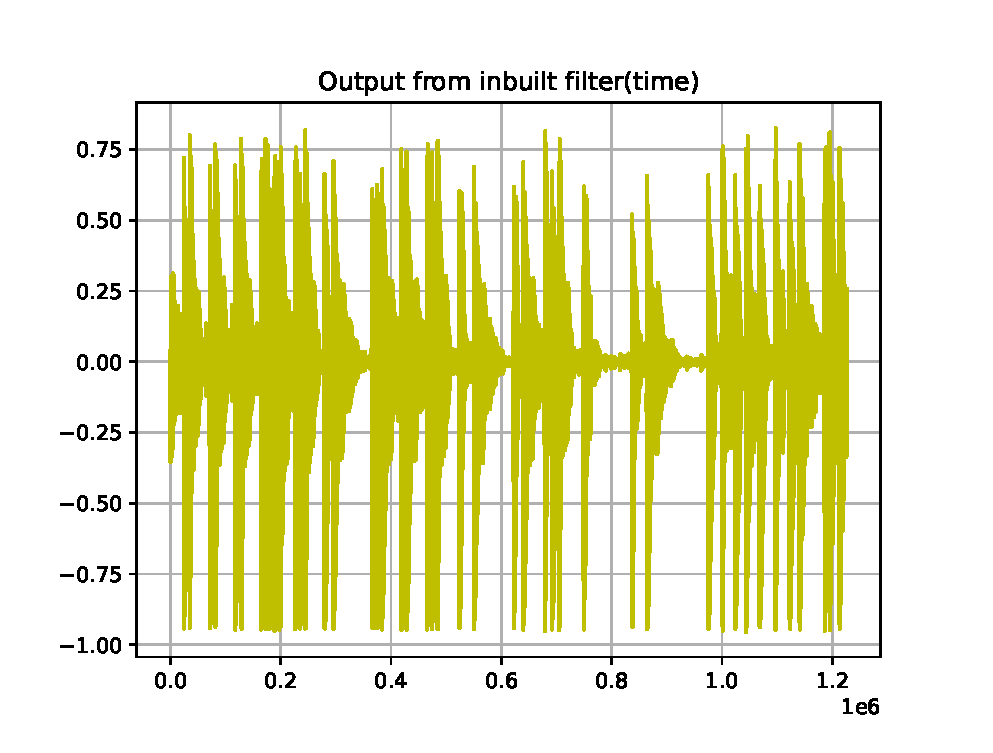
\includegraphics[width=1\columnwidth,height=0.8\columnwidth]{./figs/ee18btech11030.eps}
\caption{}
\label{fig:ee18btech11030}
\end{figure}

\begin{figure}[!ht]
\centering
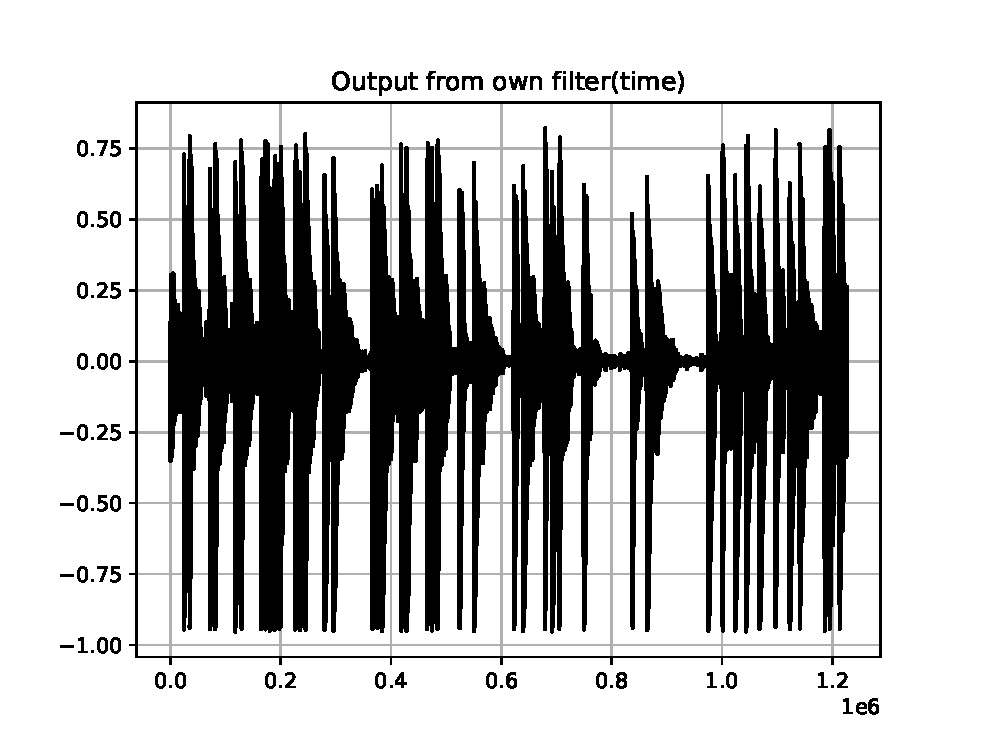
\includegraphics[width=1\columnwidth,height=0.8\columnwidth]{./figs/ee18btech11030_1.eps}
\caption{}
\label{fig:ee18btech11030_1}
\end{figure} 
\newpage

Frequency domain plots of $y(n)$ obtained using signal.filtfilt and own filter function.
\begin{figure}[!ht]
\centering
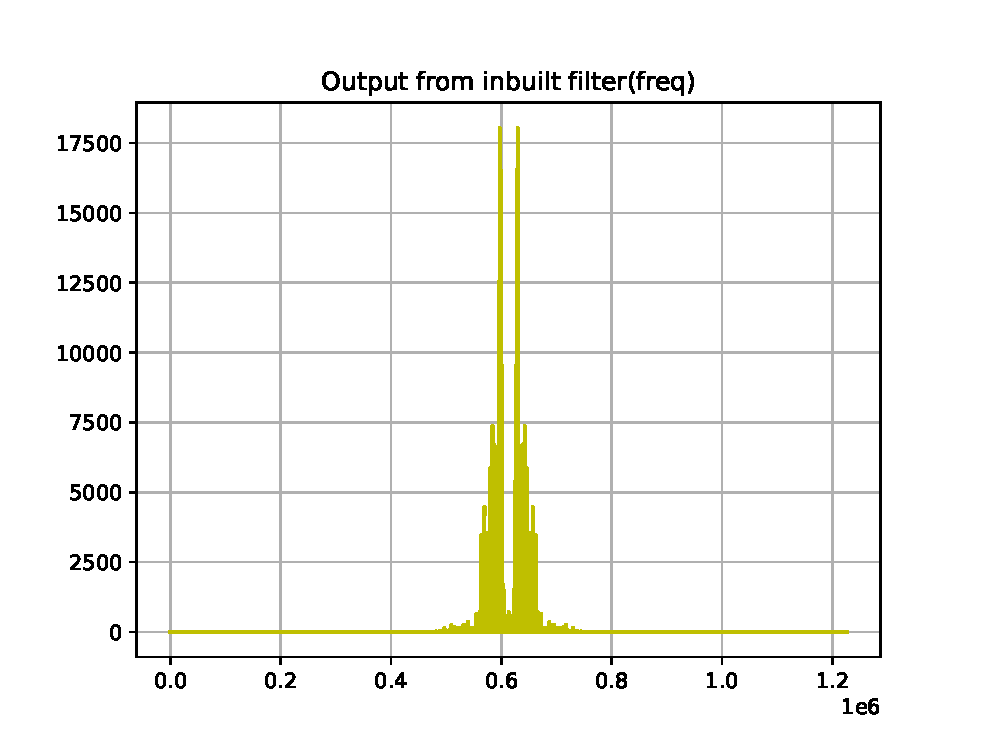
\includegraphics[width=1\columnwidth,height=0.8\columnwidth]{./figs/ee18btech11030_2.eps}
\caption{}
\label{fig:ee18btech11030_2}
\end{figure}

\begin{figure}[!ht]
\centering
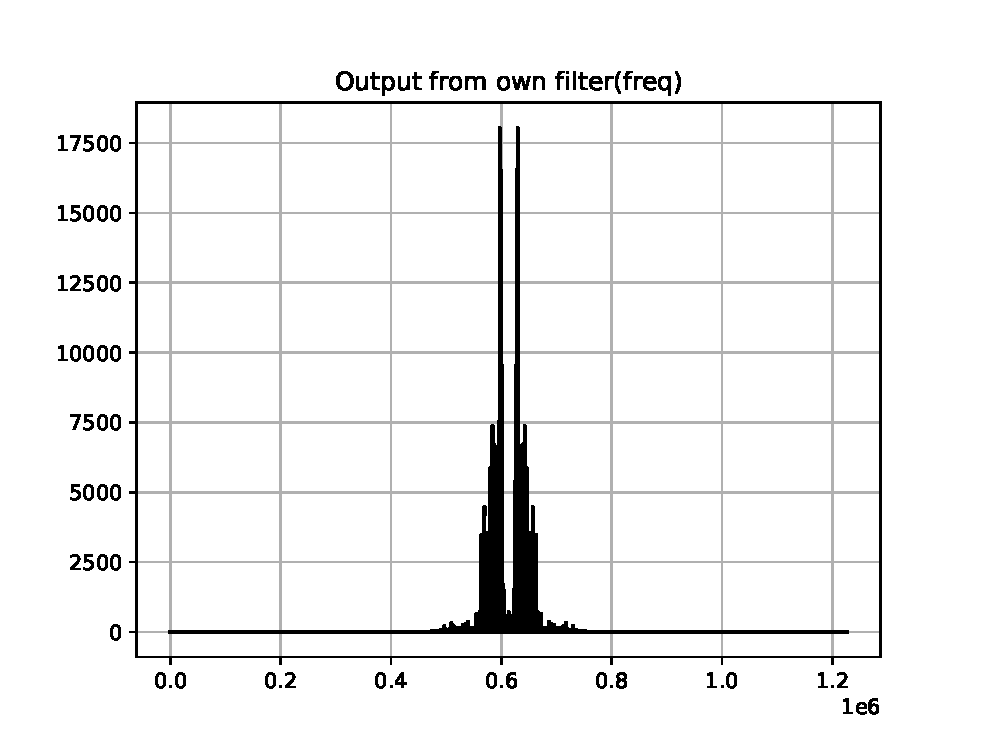
\includegraphics[width=1\columnwidth,height=0.8\columnwidth]{./figs/ee18btech11030_3.eps}
\caption{}
\label{fig:ee18btech11030_3}
\end{figure}

Below codes generate the .dat file which will be used by .c files while implementing using FFT algorthim
\begin{lstlisting}
codes/ee18btech11030_dat.py
\end{lstlisting}
codes for implementing in c
\begin{lstlisting}
codes/ee18btech11030.c
\end{lstlisting}
codes for plotting the y.dat output after implementation.
\begin{lstlisting}
codes/ee18btech11030_plot.py
\end{lstlisting}

\begin{figure}[!ht]
\centering
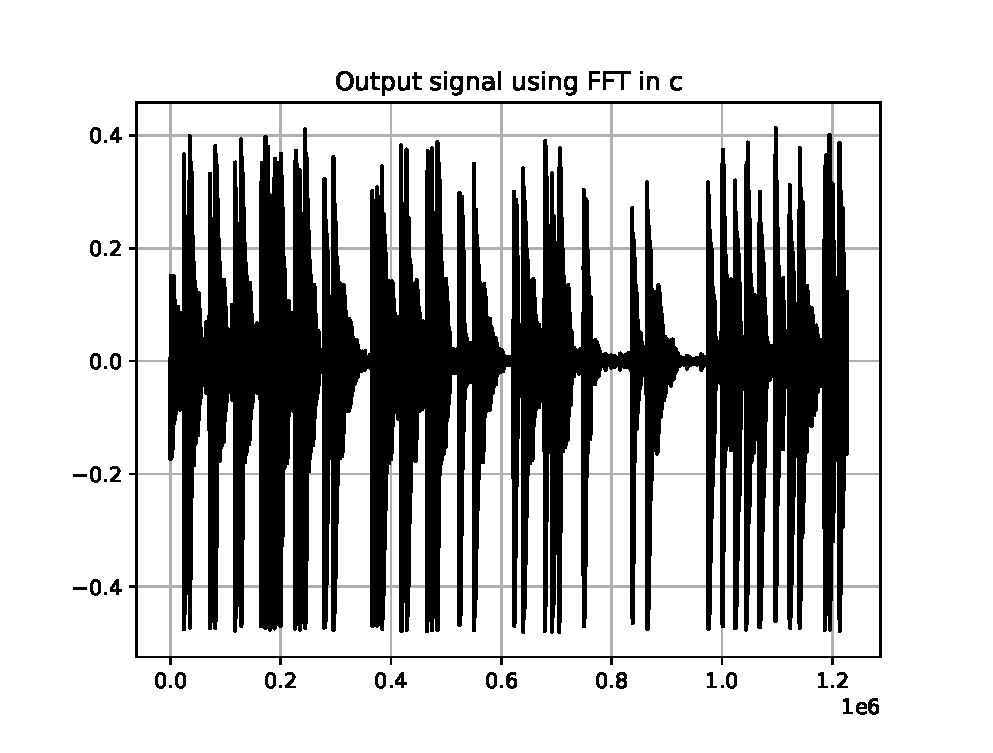
\includegraphics[width=1\columnwidth,height=0.8\columnwidth]{./figs/ee18btech11030_4.eps}
\caption{}
\label{fig:ee18btech11030_4}
\end{figure}
\end{document}
